\chapter{STUDY II - BACK SIDE DIAGNOSIS}\label{chp:Back Side Diagnosis}

In this chapter, an overview of the new pre-diagnosis (i.e., diagnosis based on back side of the foot) will be discussed—this system is based on achilles tendon. Accordingly, general system analysis and design decisions will be addressed in Section \ref{sec:StudyIIAnalysisAndDesign}. Then, specifics of implementation will be reviewed in Section \ref{sec:StudyIIImplementation}, and finally, the initial test results and evaluation phase will be discussed in Section \ref{sec:StudyIITestAndEvaluation}

\section{ANALYSIS AND DESIGN} \label{sec:StudyIIAnalysisAndDesign}

In this section, the basic structures of the system discussed in Chapter \ref{chp:Foot Detection & Primary Diagnosis} have not been changed while analyzing and designing. In addition, this chapter was profoundly focused on the small changes made to the system. Changes in requirements and design decisions will be discussed in this section.

As discussed in Section \ref{sec:StudyITestAndEvaluation}, lack of supervision causes data to be unusable and unstable test environments. Therefore, the system should be used by healthcare officials or supervised while used by participants.

\begin{figure}[htbp]
\centering
\fbox{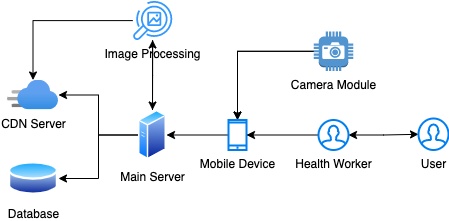
\includegraphics[width=.6\columnwidth]{KaanEksenMSc/figures/SystemOverviewStudyII.png}}
\caption{Architecture diagram of the updated system}
\label{fig:GeneralArchitectureDiagramPartI}
\end{figure}

Index results of healthcare professionals may conflict with each other due to remote image evaluations, which are discussed in Section \ref{sec:StudyITestAndEvaluation}. Therefore, healthcare professionals’ diagnosis results should be added after examinations to assess the diagnosis correctly. The general structure of the converted system can be seen in Figure \ref{fig:GeneralArchitectureDiagramPartI}.

\subsection{ Prediction And Fine Tune Module }

The prediction module consists of end-user interactions and pre-diagnosis. However, for improving results and getting more accurate test results, pre-diagnosis should be disabled since healthcare professionals will guide the participants. 

Another module, the fine-tune module, consists of background procedures and healthcare professionals' interactions. Also, the healthcare interaction module will not be used in this module since all deformities will be diagnosed on examination, and results will be entered by mobile applications. In the following paragraphs, details of the changes will be discussed.

End-user interactions on the prediction module should be updated to be usable by the healthcare professionals for supervised data collection. The same application flow should be protected except for minor modifications. For example, healthcare professionals should be able to enter the diagnosis results of the patients into the application.

In the needs analysis, the importance of the Achilles tendon in the diagnosis process was discussed with the health professionals, and therefore it was decided to base the Achilles tendon in the automated index calculation process.

\subsection{ Index Calculation }

The pre-diagnosis, the system’s underlying structure, which reduces the workload of healthcare professionals, should be updated to include rearfoot angle. The rearfoot angle is a very suitable index calculation method since it is based on the Achilles tendon.

Therefore, photographs of the back of the foot should be taken, and the rearfoot angle calculations should be made. These photos must include the calf and up to the foot's heel. In addition, legs should be centered for more accurate calculations.

\section{IMPLEMENTATION}\label{sec:StudyIIImplementation}

This section discusses the implementation details and decisions of the second study. The section focuses on changes to the modules previously discussed in section \ref{chp:Foot Detection & Primary Diagnosis}. A more detailed explanation of changes is provided by dividing it into subsections: end-user application and services and batch process.

\subsection{End-User Application}

In this section, there was no significant change in the end-user application, only minor changes have been made to improve usability. Since users are not directly using the application, some user identification options are removed, such as phone numbers. In addition, some of the optional fields for students are also removed, such as student numbers (see Figure \ref{fig:UserApplicationStudyIChanges}).

\begin{figure}[htbp]
\centering
\fbox{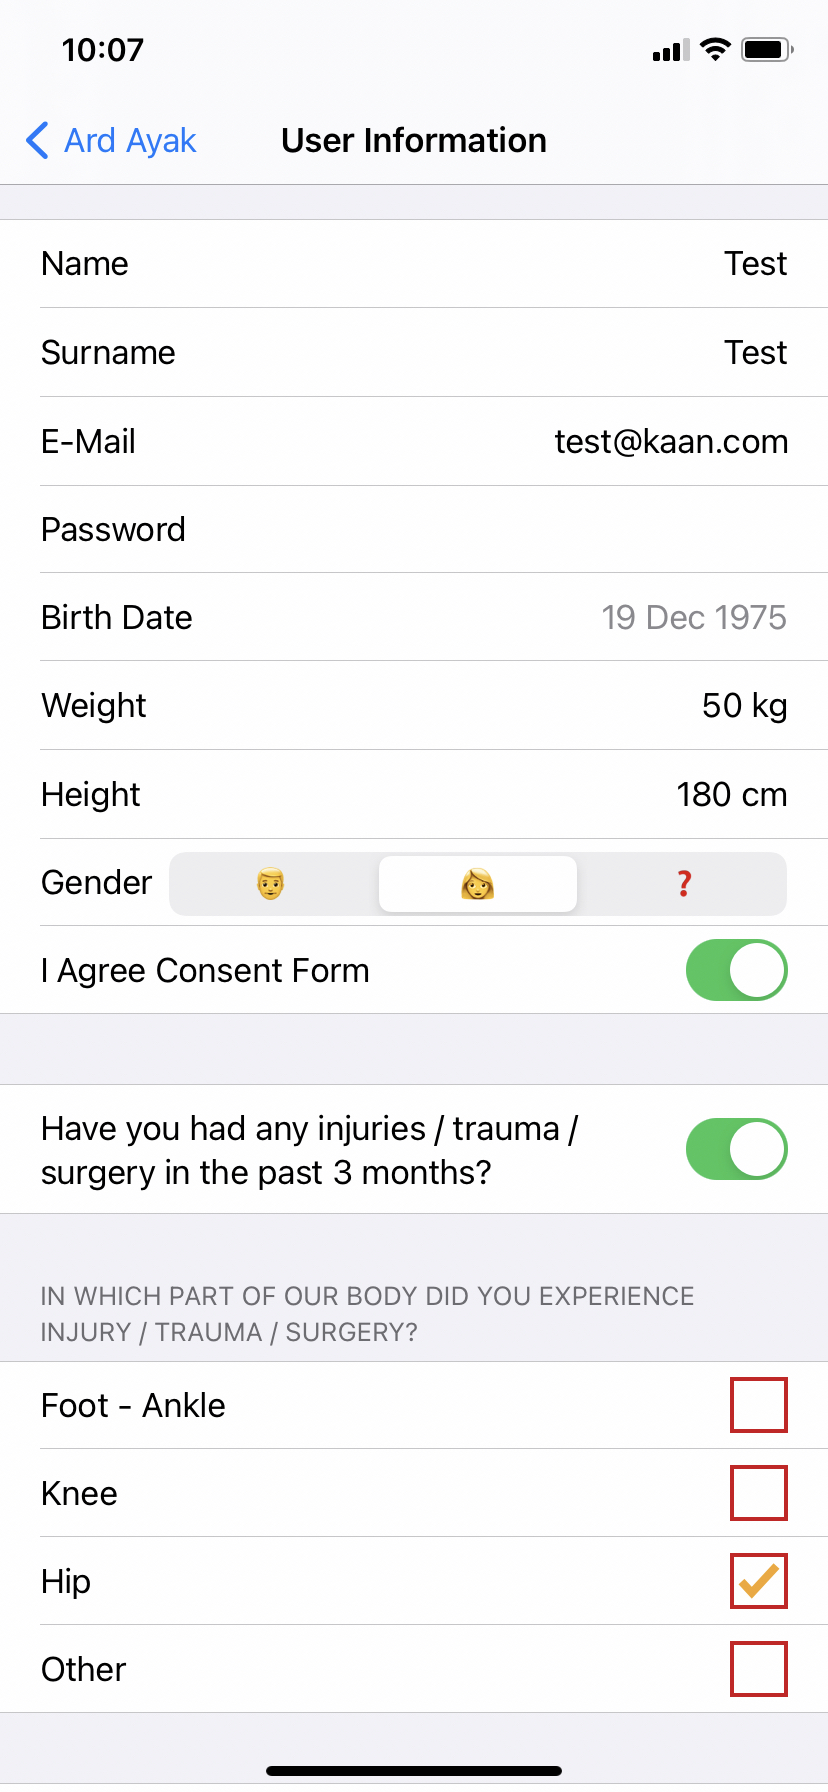
\includegraphics[width=.41\columnwidth]{KaanEksenMSc/figures/UserApplicationStudyIChanges.jpeg}}
\caption{Minor changes in end-user application in Study I}
\label{fig:UserApplicationStudyIChanges}
\end{figure}

In addition to compliance with requirements analysis, some minor bugs such as default values and crashes have been fixed, and diagnostic results have been collected as if healthcare professionals had entered them, not as if they were taken from the patient.

\subsection{Services And Batch Process}

In this section, no major changes were made to the services, except for minor adjustments and bug fixes. For the different index calculations in the automated process, most of the changes were conducted in the batch process. All these changes were explained in detail below.

One of the most significant service adjustments was made in the API. Diagnosis by option was added, which were recorded in different fields in the database (see Section \ref{sec:StudyIDatabase} for details). In addition, user type control was added to prevent misconfiguration.

\begin{figure}[htbp]
\centering
\fbox{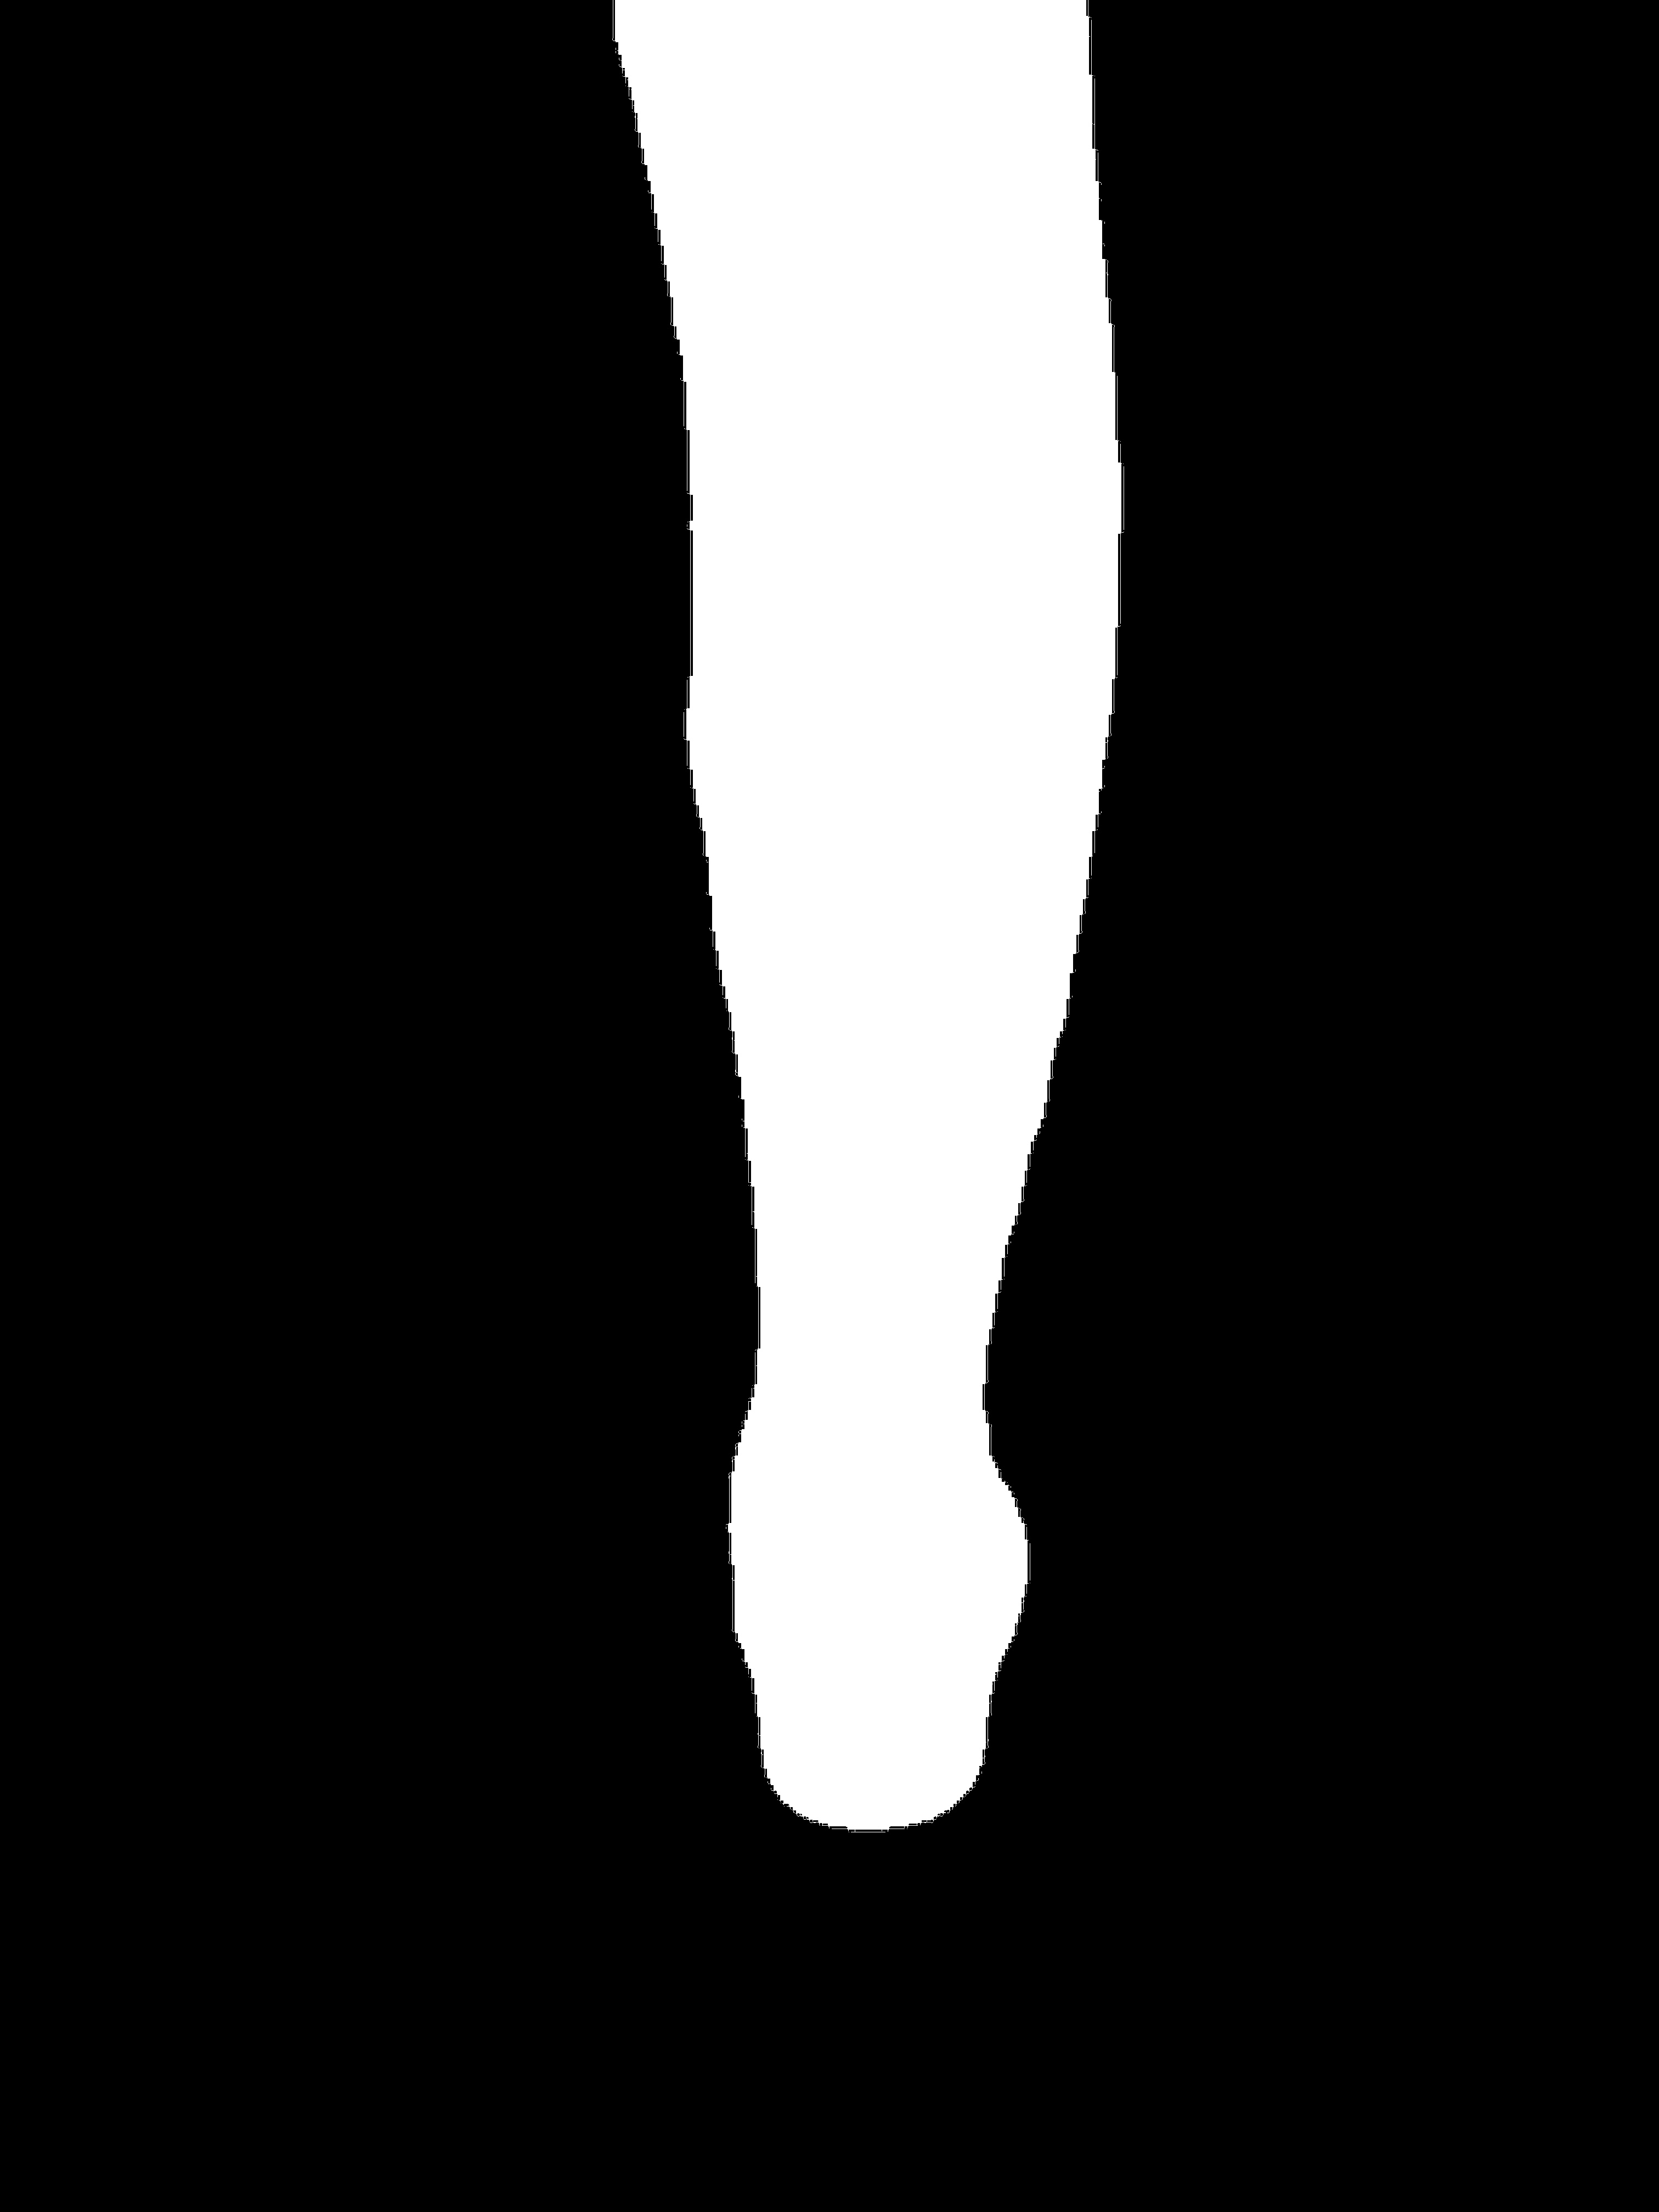
\includegraphics[width=.55\columnwidth]{KaanEksenMSc/figures/BatchProcessRioStudyII.jpeg}}
\caption{Region of interest results in Study II}
\label{fig:BatchProcessRioStudyII}
\end{figure}

The batch process calculation was redesigned from the ground up. First, the image types were differentiated so that the correct images were processed with the correct index types. Therefore, the foot-side type (see Section \ref{sec:StudyIDatabase} for details) was used to differentiate in the scan file (i.e., in the image).

After the correct image selection, the detection of the foot and leg is very important. Therefore, deep learning algorithms are applied to find the region of interest. In this study, DeepLabV3 was used to detect the region of interest, based on the experience obtained in Section \ref{sec:StudyIServicesAndBatchProcess} (see Figure \ref{fig:BatchProcessRioStudyII}).

Following the region of interest detection, critical points were detected. There are four critical points in rearfoot angle calculation (see Section for details \ref{sec:MethodologyFootDeformityDetection}). Each point requires specific points to be detected in the leg. In addition, each point is very close to the midpoint of the leg (see Figure \ref{fig:BatchProcessDotsStudyII}).

\begin{figure}[htbp]
\centering
\fbox{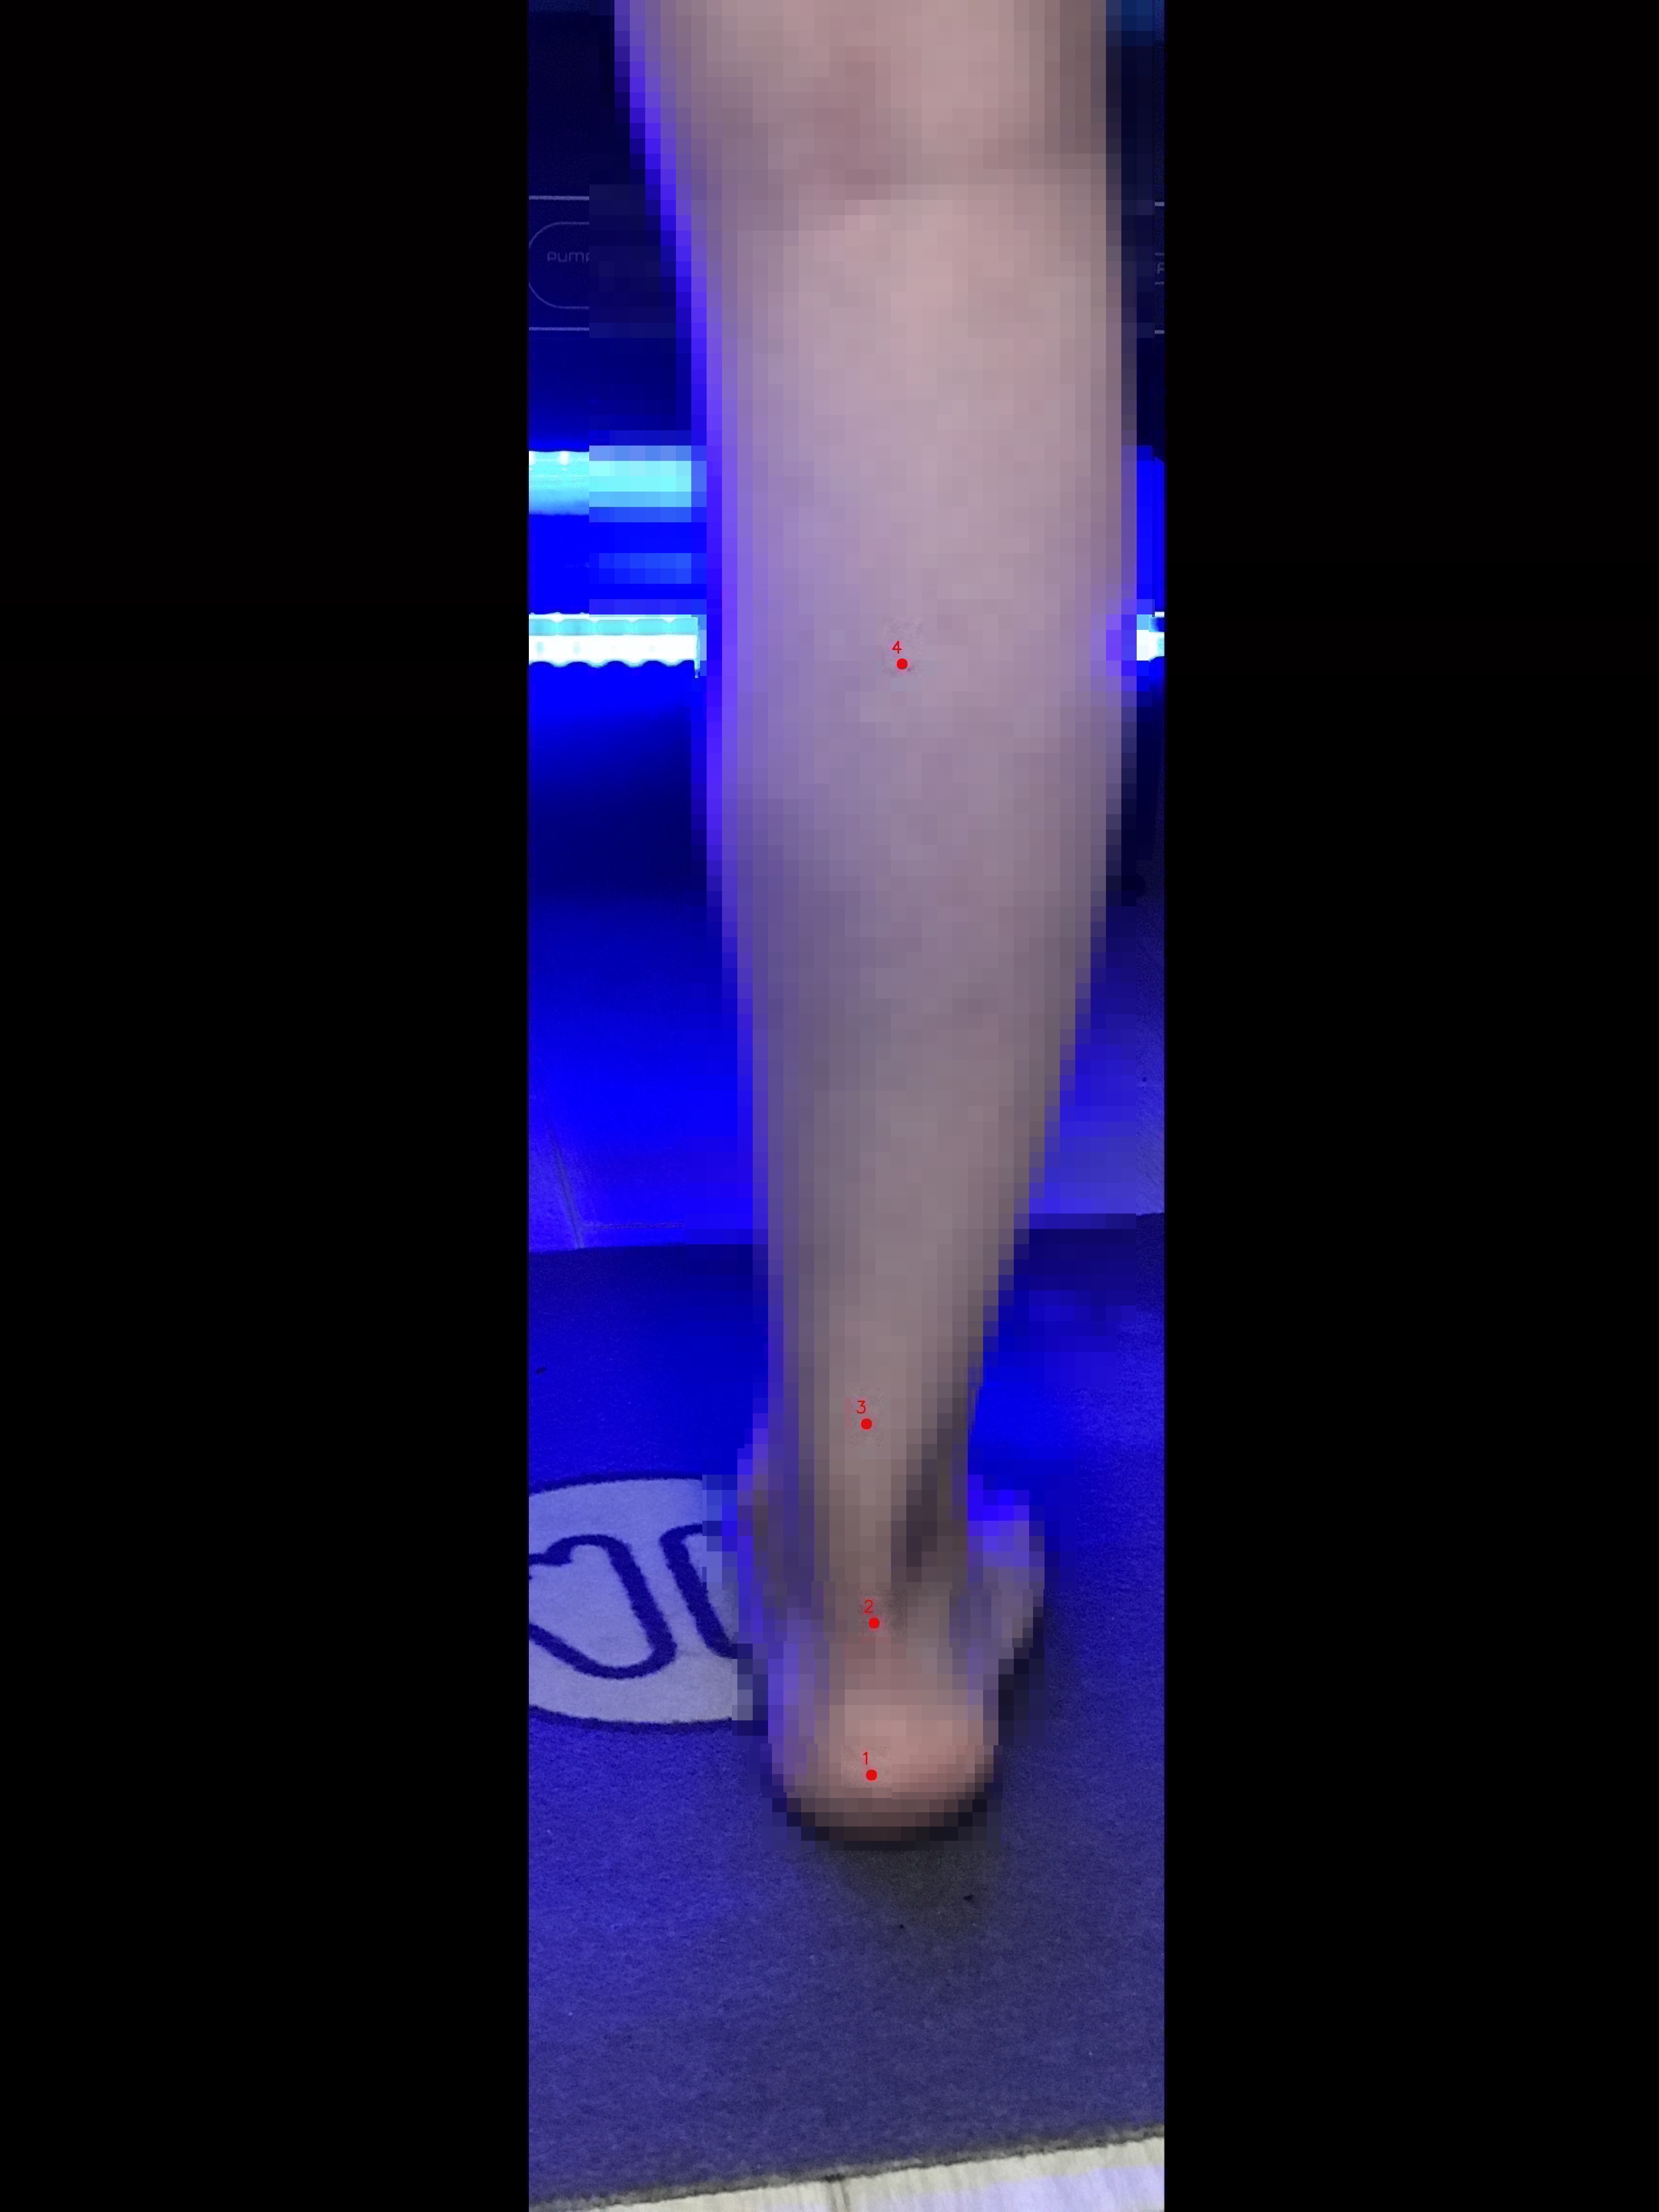
\includegraphics[width=.55\columnwidth]{KaanEksenMSc/figures/BatchProcessDotsStudyII.png}}
\caption{Calculated critical points for rearfoot angle (red dots)}
\label{fig:BatchProcessDotsStudyII}
\end{figure}

The first point base of the calcaneus is calculated based on the region of interest. Processing is started from the bottom of the image, where the initial region is detected, wideness of the foot area is recorded. In case of the region of interest errors, the processing is continued until 30 percent of the image width from the initial region detection. If new wideness is more significant than 50 percent of the initial detection, new area wideness is considered the calcaneus's base.

The second point determination is based on the assumption that the ankle is the thinnest area in the leg. Therefore, the narrowing of the leg is sought, following the first point discovery. After this region is found, the point that is 5 percent below the region of interest is considered as the second breakpoint. In addition, the third point had a similar discovery process. The only difference is that the third point is 5 percent up by the region of interest

The fourth point corresponds to the narrowing point of the calf. Therefore, after the third point was found, narrowing was sought in the region.

\section{TEST AND EVALUATION}\label{sec:StudyIITestAndEvaluation}

In this section, the test and evaluation process of the prototype system, which is explained in detail in the previous sections, will be discussed.

\begin{table}[htbp]
\begin{center}
\caption{Participant statistics in study II}
\vspace{23pt}
      \begin{tabular}{|c|c|c|c|c|} \hline
          & \textbf{Age} & \textbf{Weight} & \textbf{Height} & \textbf{BMI} \\ \hline
        \textbf{Avarage} & 22.67 & 70.89 & 173.11 & 23.24 \\ \hline
        \textbf{Max} & 29 & 100 & 190 & 30.19 \\ \hline
        \textbf{Min} & 21 & 50 & 159 & 19.05 \\ \hline
    \end{tabular}
\label{tab:StudyIIParticipantStatistics}
\end{center}
\end{table}

In the second study, test data are collected through mobile applications under the supervision of healthcare professionals. Therefore, the collected data are evaluated before the procedure. In addition, a document describing how to use the application was given to the healthcare professionals.

The prototype was used by 9 participants, where 3 (33.33 percent) of them were female, and the remaining 6 (66,67 percent) were male, with an average age of 22.6 (see Table \ref{tab:StudyIIParticipantStatistics} for details). Data was stored in an online database which is described in section \ref{sec:StudyIAnalysisAndDesign}.

\begin{figure}[htbp]
\centering
\fbox{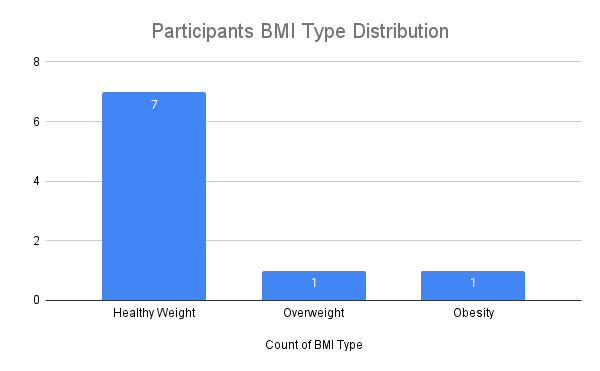
\includegraphics[width=.65\columnwidth]{KaanEksenMSc/figures/StudyIIParticipantsBMITypeDistribution.png}}
\caption{Participants BMI type distribution based on CDC in study II}
\label{fig:StudyIIParticipantsBMITypeDistribution}
\end{figure}

BMI is critical as most index calculations are based on the ratio to eliminate the effects of weight. Population's average BMI is 23.2 (healthy weight), (see Figure \ref{fig:StudyIIParticipantsBMITypeDistribution}). Therefore, this might not provide sufficient data for projection in different wight scales.

\begin{figure}[htbp]
\centering
\fbox{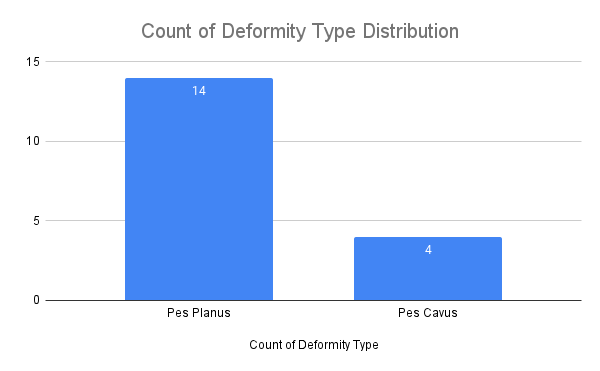
\includegraphics[width=.60\columnwidth]{KaanEksenMSc/figures/StudyIIFootDeformityTypeDistribution.png}}
\caption{Foot deformity type distribution in study II}
\label{fig:StudyIIFootDeformityTypeDistribution}
\end{figure} 

All 18 photos collected in the application were used because during the collection of photos all users are supervised by healthcare professionals. In addition, deformety types of the users were validated in the examination by healthcare professionals before sended to the system (see Figure  \ref{fig:StudyIIFootDeformityTypeDistribution}).

\begin{figure}[htbp]
\centering
\fbox{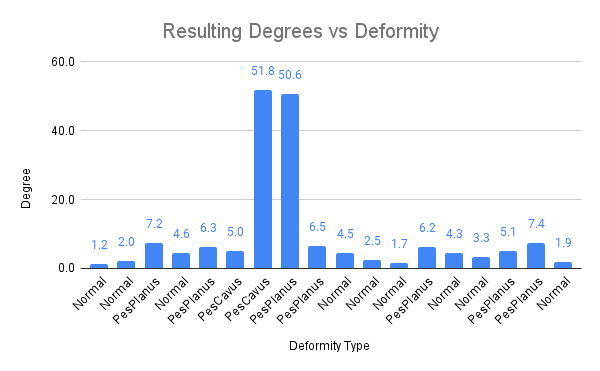
\includegraphics[width=.60\columnwidth]{KaanEksenMSc/figures/StudyIIFootDeformityAutomatedDegreesAndDeformityResults.png}}
\caption{Rear foot angle vs foot deformity in automated process results}
\label{fig:StudyIIFootDeformityAutomatedDegreesAndDeformityResults}
\end{figure} 

After the data collection, automated index calculations are conducted. Initial results showed that the findings of the healthcare officials and the system were 27,7 percent matched. This low performance may be caused by multiple factors such as image angle, color disorientation, assumptions in point location determination. However, it was thought that the biggest effect in the evaluations was the sensitivity of the Rear foot angle to the calculation error. Because this calculation only determines the deformity according to a difference of 5 degrees. It is very difficult to detect this 5 degree difference in the photos taken via the mobile application (see Figure \ref{fig:StudyIIFootDeformityAutomatedDegreesAndDeformityResults}). 
